%%%%%%%% ICML 2021 EXAMPLE LATEX SUBMISSION FILE %%%%%%%%%%%%%%%%%

\documentclass{article}
\usepackage[utf8]{vietnam}
\usepackage[vietnam]{babel}
% Recommended, but optional, packages for figures and better typesetting:
\usepackage{microtype}
\usepackage{graphicx}
\usepackage{subfigure}
\usepackage{booktabs} % for professional tables
\usepackage{multicol}
\usepackage{svg}
\usepackage{natbib} 
\usepackage{amsmath}
\setcitestyle{square,semicolon}
\usepackage{hyperref}
\hypersetup{
    colorlinks=true,
    linkcolor=blue,
    filecolor=magenta,      
    urlcolor=red,
    pdftitle={Overleaf Example},
    pdfpagemode=FullScreen,
}
\usepackage{pgfplots}
\usepackage{tikz} 

% Attempt to make hyperref and algorithmic work together better:
\newcommand{\theHalgorithm}{\arabic{algorithm}}

\usepackage[accepted]{icml2021}

% The \icmltitle you define below is probably too long as a header.
% Therefore, a short form for the running title is supplied here:

\icmltitlerunning{Dự đoán áp lực của máy thở bằng XGBoost}
\begin{document}
% \icmltitle{Submission and Formatting Instructions for ICML 2021}

\twocolumn[

\icmltitle{Dự đoán áp lực của máy thở bằng XGBoost}

\begin{icmlauthorlist}
\icmlauthor{Bùi Trí Dũng}{to}
\icmlauthor{Võ Khánh An}{to}
\icmlauthor{Phạm Ngọc Tân}{to}
\end{icmlauthorlist}

\icmlcorrespondingauthor{Bùi Trí Dũng}{19521386@gm.uit.edu.vn}
\icmlcorrespondingauthor{Võ Khánh An}{19520007@gm.uit.edu.vn}
\icmlcorrespondingauthor{Phạm Ngọc Tân}{19520925@gm.uit.edu.vn}


\icmlaffiliation{to}{Trường Đại học Công nghệ Thông tin, ĐHQG HCM}

% \icmlcorrespondingauthor{a}{c.vvvvv@googol.com}
% \icmlcorrespondingauthor{Eee Pppp}{ep@eden.co.uk}

% You may provide any keywords that you
% find helpful for describing your paper; these are used to populate
% the "keywords" metadata in the PDF but will not be shown in the document
\icmlkeywords{Machine Learning, XGBoost}

\vskip 0.3in
]

% this must go after the closing bracket ] following \twocolumn[ ...

% This command actually creates the footnote in the first column
% listing the affiliations and the copyright notice.
% The command takes one argument, which is text to display at the start of the footnote.
% The \icmlEqualContribution command is standard text for equal contribution.
% Remove it (just {}) if you do not need this facility.

%\printAffiliationsAndNotice{}  % leave blank if no need to mention equal contribution
\printAffiliationsAndNotice{\icmlEqualContribution} % otherwise use the standard text.

\begin{abstract}
Hiện nay, đại dịch COVID-19 vẫn đang diễn biến phức tạp và gây ra những hậu quả vô cùng nặng nề. Những bệnh nhân bị trở nặng cần phải sử dụng máy thở dưới sự điều chỉnh và giám sát từ các nhân viên y tế có chuyên môn. Tuy vậy, việc số ca nhiễm tăng lên theo cấp số nhân tại một số khu vực trên thế giới đã đẩy hệ thống y tế rơi vào tình trạng quá tải. Do đó, việc xây dựng những máy thở có thể tự động điều chỉnh thông số trong quá trình điều trị là một việc làm vô cùng thiết thực trong giai đoạn này. Trong bài này, chúng tôi sẽ tiến hành dự đoán áp lực của máy thở lên bệnh nhân qua những thông số của máy thở và tình trạng của bệnh nhân bằng thuật toán XGBoost. Bên cạnh các kỹ thuật học sâu, XGBoost là một thuật toán nhằm giải quyết các bài toán học có giám sát cho độ chính xác khá cao và đã đạt nhiều chiến thắng trong các cuộc thi trên Kaggle. Hơn thế nữa, XGBoost còn có tốc độ huấn luyện nhanh và khả năng tính toán song song nhằn tận dụng sức mạnh của GPU. Tất cả những nghiên cứu của chúng tôi đều được công khai tại: \url{https://github.com/DTA-UIT/Ventilator_Pressure_Prediction}

\end{abstract}


\section{Giới thiệu} 
% XGBoost hiện nay đã trở thành một trong những công cụ được sử dụng rộng rãi và thực sự phổ biến giữa các đối thủ khi cạnh tranh với những cuộc thi trên Kaggle và các đối với nhà khoa học thiên về dữ liệu trong ngành, vì nó đã được thử nghiệm trong nhiều vấn đề có quy mô lớn. XGboost là một công cụ được đánh giá rất linh hoạt và \textbf{có thể giải quyết hầu hết các bài toán liên quan đến hồi quy (regression), phân loại (classification) và xếp hạng (ranking)}. 

% XGBoost là tên viết tắt của \textbf{Extreme Gradient Boosting}, được phát triển bởi Tianqi Chen và hiện là một phần của bộ sưu tập thư viện mã nguồn mở rộng và đang được phát triển bởi Cộng đồng Máy học Phân tán (DMLC). XGBoost có thể triển khai chính xác hầu hết các mục tiêu mà con người đặt ra cũng như đã chứng minh được sức mạnh của nó. 

% Hầu hết trong các cuộc thi liên quan đến Kaggle thì việc lựa chọn thư viện cũng như mô hình cũng được xem là bước quan trọng nhằm đánh giá độ chính xác và tốc độ của thực thi của mô hình. Tính năng chính của thư viện XGBoost chính là giúp cải thiện độ thực thi huấn luyện mô hình và tỉ lệ chính xác tương đối của bài toán được đặt ra.. 



Thông thường, khi một bệnh nhân gặp phải các vấn đề về hô hấp thì các bác sĩ sẽ tiến hành sử dụng máy thở để bơm Oxy vào bên trong phổi của bệnh nhân thông qua một đường ống được luồng vào khí quản. Tuy nhiên, việc sử dụng thành thạo máy thở là một công việc đòi hỏi rất nhiều kiến thức y khoa. Điều này là một trở ngại cực lớn trong bối cảnh tình hình đại dịch COVID-19 ngày càng trở nên căng thẳng tại nhiều quốc gia trên thế giới, dẫn đến hệ thống y tế bị quá tải và nhiều nơi không có đủ nguồn nhân lực là nhân viên y tế có chuyên môn trong việc điều chỉnh máy thở. Mặt khác, việc phát triển những công nghệ mới để có thể vận hành được máy thở y tế thường sẽ rất tốn kém và bị giới hạn về mặt y học. Vì vậy, việc dự đoán áp lực thở sẽ giúp các bác sĩ mô phỏng lại quá trình điều chỉnh các thông số. Qua đó giúp phá vỡ đi những rào cản hiện tại.

Từ trước tới nay đã có nhiều kỹ thuật và thuật toán trong học máy được đề xuất để giải nhiều bài toán nhằm tiết kiệm nguồn nhân lực là các chuyên gia trong ngành y tế. Một trong số đó phải kể đến các thuật toán thuộc lớp Gradient Tree Boosting \cite{gradient-boosting} - một nhánh của họ thuật toán cây quyết định tổng hợp (ensemble decision tree) sử dụng phương pháp Boosting để gia tăng độ chính xác cho dữ liệu đầu ra. Phương pháp Boosting đã được kiểm chứng rộng rãi với những kết quả state-of-the-art trên nhiều benchmark khác nhau \cite{sota-xgboost}. Ngoài ra, các thuật toán Tree-boosting còn được các kỹ sư phần mềm áp dụng trong việc thiết kế ra các pipeline thích hợp tạo nên những trải nghiệm tích cực hơn cho người dùng web \cite{example1}.
\begin{center} 
\begin{figure}[!h]
    \centering
    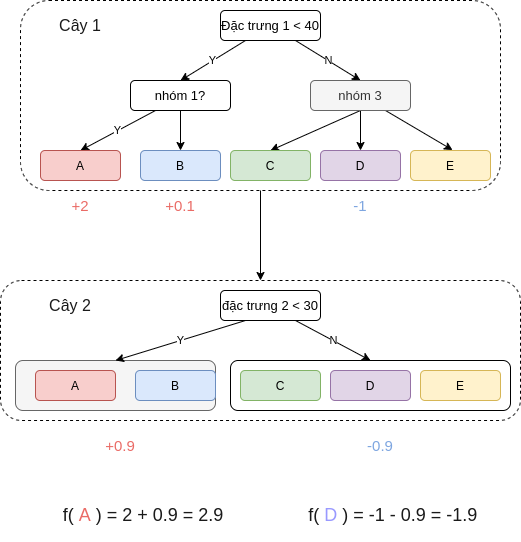
\includegraphics[scale=0.4]{graph-Page-1.drawio.png}
    \caption{Ví dụ về cây quyết định tổng hợp\\với dữ liệu đầu ra là tổng của các dự đoán từ các cây quyết định}
    \label{fig:Viducayquyetdinh}
\end{figure}
\end{center}
Trong bài báo cáo này, chúng tôi sẽ giới thiệu XGBoost \cite{xgboost}, một thuật toán máy học có thể thích nghi (scalable machine learning system) nằm trong họ thuật toán Tree-boosting. XGBoost đã được chứng tỏ được tính ổn định và độ chính xác trong nhiều cuộc thi về học máy và khai phá dữ liệu. Ngoài ra, XGboost còn là một công cụ được đánh giá rất linh hoạt và có thể giải quyết hầu hết các bài toán liên quan đến hồi quy (regression), phân loại (classification) và xếp hạng (ranking). Cụ thể hơn, khi vừa mới được giới thiệu vào năm 2014, XGBoost đã đem lại chiến thắng cho 17 đội trên tổng số 29 cuộc thi trên Kaggle chỉ trong năm 2015. Trong số 17 đội chiến thắng sử dụng XGBoost, chỉ có 8 đội sử dụng mô hình XGBoost đơn thuần, 9 đội còn lại chọn cách kết hợp XGBoost với các kỹ thuật học máy khác.

Trong bài nghiên cứu này, chúng tôi sẽ tiến hành giới thiệu về các công trình liên quan đến phạm vi của XGBoost ở phần 2. Sau đó, chúng tôi sẽ đưa ra nền tảng của XGBoost ở phần 3 và bàn luận chi tiết về thuật toán XGBoost cũng như các ưu, nhược điểm của nó ở phần 4. Hai phần tiếp theo sẽ được tập trung để nói về cách chúng tôi thiết kế thực nghiệm thông qua giới thiệu và phân tích tập dữ liệu được sử dụng (phần 5) cũng như chi tiết về độ đo, chi tiết triển khai, kết quả đạt được và triển khai ứng dụng (phần 6). Sau cùng, chúng tôi sẽ bàn luận mở rộng về XGBoost và đưa ra những bàn luận và kết luận cuối cùng về XGBoost ở phần 7 và 8.



% /----------------------------------/
% \section{Các phần liên trong trong XGBoost }

% \subsection{Regularized Learning Objective}
% Giả sử rằng mô hình nhận được một tập dữ liệu gồm $n$ mẫu trong đó chứa $m$ đặc trưng $\mathcal{D} = \{ \left( x_{i}, y_{i}\right) \}  \left( | \mathcal{D} | = n, x_{i} \in \mathcal{R}^{m}, y_{i} \in \mathcal{R}  \right)$, một mô hình cây tổng hợp được minh họa như trong hình \ref{fig:Viducayquyetdinh} sử dụng $K$ hàm tính toán để dự đoán đầu ra của mô hình: 
% \begin{center}
%     \begin{math} 
%         \hat{y}_{i} = \phi(x_{i}) = \sum^{K}_{k=1}{f_k(x_{i})}, f_{k} \in \mathcal{F}
%     \end{math}
% \end{center}
 
% Biết rằng $\mathcal{F} = \{ f(x) = w_{q(x)}\} (q : \mathcal{R}^{m} \rightarrow \mathcal{T}, w \in \mathcal{R}^{\mathcal{T}})$ chính là không gian của cây hồi quy hay còn biết đến với tên viết tắt CART. $q$ đại diện cho cấu trúc của mỗi cây - được xây dựng lên từ các lá. $\mathcal{T}$ là số lượng lá trong mỗi cây. Với mỗi hàm $f_{k}$ sẽ đại diện cho mỗi một cấu trúc cây một cách độc lập $q$ và trọng số của nút lá $w$. 

% Khác với decision tree, mỗi một cây hồi quy biểu diễn score trên mỗi nút lá bằng cách xem $w_{i}$ là score trên mỗi một lá thứ $i$. Như ví dụ hình bên trên, mô hình sẽ sử dụng quy luật quyết định trên các cây (được quy định bởi $q$) để phân loại thành nhiều nút lá khác nhau và tính toán ra kết quả đầu ra cuối cùng bằng tổng các score tương ứng với mỗi nút lá (được quy định bởi $w$). 
 
% \begin{center}
%     \begin{equation}
%         \mathcal{L} (\phi) = \sum_{i} l(\hat{y_{j}}, y_{i}) + \sum_{k}\Omega(f_k)
%     \end{equation}  
% \end{center}

% \begin{center} 
%     \begin{equation} 
%         \Omega(f) = \gamma\mathcal{T} + \frac{1}{2} \lambda\|w\|^{2}
%     \end{equation}
% \end{center}
 
% Với $l$ chính là sai số giữa $\hat{y}$ và $y$. Thành phần thứ hai chính là $\Omega$ có chức năng tăng mức phạt cho mô hình. Ngoài ra thành phần chính quy hóa giúp cho mô hình có thêm độ "smooth" trong việc học các trọng số để tránh hiện tượng over-fitting. Theo một cách trực quan, mục tiêu của hàm chính quy hóa thường sẽ chú trọng đến việc lựa chọn một mô hình đơn giản và hàm dự đoán của mô hình hơn. Một trong các công nghệ về chính quy hóa tương tự của mô hình này đã được sử dụng trong mô hình Regularized greedy forest (RGF). Tuy nhiên trong mô hình XGBoost, tác giả sử dụng hàm mục tiêu và thuật toán học đơn giản và dễ hơn so với RGF nhằm mục đích xây dựng hệ thống song song. 
 
% \subsection{Gradient Tree Boosting}

% Gọi $\hat{y_{i}}^{(t)}$ là đầu ra dự đoán của tại ở mẫu thứ $i$ lần lặp thứ $t$ se được cộng thêm giá trị hàm $f_t$ để cực tiểu hóa hàm mục tiêu như sau:

% \begin{center}
%     \begin{equation} 
%         \mathcal{L}^{(t)} = \sum^{n}_{i=1} l\left( y_{i}, \hat{y_{y}}^{t-1} + f_{t}(x_{i})\right) + \Omega(f_{t})
%     \end{equation}
% \end{center}

% Việc công thêm giá trị hàm $f_t$ sẽ làm cải thiện độ chính xác của mô hình. Xấp xỉ đạo hàm bậc 2 có thể được sử dụng cho việc tối ưu hàm mục tiêu một cách nhanh chóng hơn: 

% \begin{center}
%     \begin{equation}  
%         \mathcal{L}^{(t)} \approx \sum^{n}_{i=1} [ l( y_{i}, \hat{y}^{(t - 1)} ) + g_{i}f_{t}(x_{i}) + \frac{1}{2} h_{i}f_{t}^{2}(x_{i}) ] + \Omega\left(f_{t}\right)
%     \end{equation}
% \end{center}

% Với $g_{i} = \partial_{\hat{y}^{(t-1)}}l( y_{i}, \hat{y}^{(t - 1)})$ và $h_{i} = \partial^{2}_{\hat{y}^{(t - 1])}} l(y_{i}, \hat{y}^{(t - 1)}$ tương ứng với đạo hàm bậc một và đạo hàm bậc hai của hàm mất mát. Đồng thời có thể bỏ qua phần hằng số để mô hình có thể đơn giản hơn cho hàm mục tiêu tại bước thứ $t$.

% \begin{center}
%     \begin{equation}  
%         \mathcal{L}^{(t)} = \sum^{n}_{i=1} [ g_{i}f_{t}(x_{i}) + \frac{1}{2} h_{i}f_{t}^{2}(x_{i}) ] + \Omega\left(f_{t}\right)
%     \end{equation}
% \end{center}

% \begin{center} 
% \begin{figure}[!h]
%     \centering
%     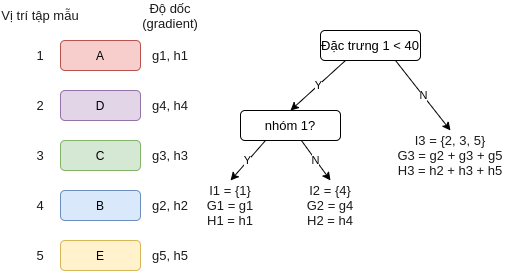
\includegraphics[scale=0.45]{graph-Page-2.drawio (2).png}
%     \caption{Mô phỏng cấu trúc tính score của XGBoost}
%     \label{fig:StructScoreCalculation}
% \end{figure}
% \end{center}

% Đặt $\mathcal{I}_{j} = \{ i | q_{(x_{i})} = j\}$ là tập mẫu tại nút lá thứ $j$. Có thể mở rông công thức trên với $\Omega$ như sau: 

% \begin{center} 
%     \begin{align*} 
%         \mathcal{L}^{(t)} &= \sum^{n}_{i=1} \left[ g_{i}f_{t}(x_{i}) + \frac{1}{2} h_{i}f_{t}^{2}(x_{i}) \right] + \gamma\mathcal{T} + \frac{1}{2}\lambda\sum_{j=1}^{\mathcal{T}} {w_{j}^{2}} \\ 
%         &= \sum^{\mathcal{T}}_{j=1}\left[ \left( \sum_{i \in \mathcal{I}_{j} } g_{i} \right) w_{j} + \frac{1}{2} \left( \sum_{i \in \mathcal{I}_{j}}{h_i} + \lambda \right)w_{j}^{2} \right] + \gamma\mathcal{T}
%     \end{align*}
% \end{center}

% Bởi vì cấu trúc $q(x)$ là một cấu trúc cố định, do đó có thể tính toán được trọng số tối ưu $w^{*}_{j}$ tại nút lá thứ $j$ bằng cách: 

% \begin{center}
%     \begin{equation}  
%         w_{j}^{*} = - \frac{\sum_{i \in \mathcal{I}_{j}} g_{i}}{\sum_{i \in \mathcal{I}_{j}} +  h_{i} + \lambda}
%     \end{equation}
% \end{center} 

% và tính toán giá trị tối ưu tương ứng: 

% \begin{center}
%     \begin{equation}  
%         \mathcal{L}^{(t)}(q) = - \frac{1}{2} \sum_{j=1}^{\mathcal{T}} \frac{\sum_{i \in \mathcal{I}_{j}} g_{i}}{\sum_{i \in \mathcal{I}_{j}} +  h_{i} + \lambda} + \gamma\mathcal{T}
%         \label{eq:score}
%     \end{equation}
% \end{center} 

% Từ công thức số \ref{eq:score} có thể dùng như hàm scoring - ước tính chất lượng của một cấu trúc $q$. Hình ảnh số \ref{fig:StructScoreCalculation} sẽ mô phỏng rõ hơn về việc tính $score$ của mô hình trên một cây bất kì. 

% Theo cách thông thường hầu như sẽ không thể liệt kê tất cả các cấu trúc cây $q$. Thuật toán tham lam bắt đầu từ một lá và thêm các nhánh một cách lần lượt trên cây. Giả sử rằng $\mathcal{I}_{L}$ và $\mathcal{I}_{R}$ là hai tập mẫu của nút lá trái và nút lá phải sau khi được chia thành hai nhánh riêng biệt.

% % \begin{center} 
%     \begin{align*} 
%         \mathcal{L}_{split} = \frac{1}{2} \left[ \frac{\left(\sum_{i \in \mathcal{I}_{L}}{g_{i}} \right)^2}{ \sum_{i \in \mathcal{I}_{L}}{h_{i} + \lambda}} + \frac{\left(\sum_{i \in \mathcal{I}_{R}}{g_{i}} \right)^2}{ \sum_{i \in \mathcal{I}_{R}}{h_{i} + \lambda}} - \frac{\left(\sum_{i \in \mathcal{I}}{g_{i}} \right)^2}{ \sum_{i \in \mathcal{I}}{h_{i} + \lambda}}\right] - \gamma 
%     \end{align*} 
% % \end{center} 

% Công thức trên thường được sử dụng trong thực để để đánh giá các ứng cử viên sau khi tách thành các nhánh các khau. 


% https://arxiv.org/pdf/1603.02754.pdf
\section{Các công trình liên quan}
% /----------------------------------/
% XGBoost là một thuật toán học máy dựa trên cây tổng hợp sử dụng gradient boosting framework. 
Các thuật toán gradient boosting đang dần trở nên phổ biến đối với dữ liệu dạng bảng. Trong những năm vừa qua, chúng ta đã chứng kiến rất nhiều thuật toán boosting ra đời, mỗi thuật toán lại có những đặc điểm riêng biệt. Cụ thể, các thuật toán khác nhau ở việc triển khai cũng như tính tương thích và hạn chế về mặt kỹ thuật của chúng. XGBoost là thuật toán Gradient Boosting Machine (GBM) đầu tiên cải thiện đáng kể thời gian huấn luyện. Tiếp theo là LightGBM \cite{lightgbm} và CatBoost \cite{catboost}, mỗi thuật toán có các kỹ thuật riêng, chủ yếu liên quan đến cơ chế phân tách (spliting mechanism). Các bản cập nhật của những thuật toán này liên tục được ra mắt với nhiều tính năng và khiến chúng ngày càng mạnh mẽ hơn. 

% /----------------------------------/
\section{Nền tảng}
\subsection{Boosting}
Boosting được hiểu đơn giản là tăng hiệu quả của mô hình. Trong học máy, boosting là một kỹ thuật học tổng hợp (ensemble learning) để chuyển đổi một giả thuyết yếu thành mạnh để làm tăng độ chính xác của mô hình. 

Những quy tắc yếu được tạo ra ở mỗi vòng lặp bởi các thuật toán học cơ sở (base learning algorithms), thứ có thể được chia làm 2 loại: mô hình dựa trên cây (tree-based learner) và mô hình dựa trên tuyến tính (linear-based learner). Nói chung, cây quyết định là mô hình cơ sở (base learner) mặc định của boosting.

\subsection{Học tổng hợp}
Học tổng hợp (ensemble learning) \cite{ensemblelearning} là một quá trình mà trong đó các quyết định từ nhiều mô hình học máy được kết hợp để giảm lỗi và cải thiện việc dự đoán khi so sánh một mô hình học máy đơn. Sau đó kỹ thuật biểu quyết tối đa (maximum voting) được sử dụng trên các cây quyết định tổng hợp để suy ra dự đoán cuối cùng.

\begin{center} 
\begin{figure}[!h]
    \centering
    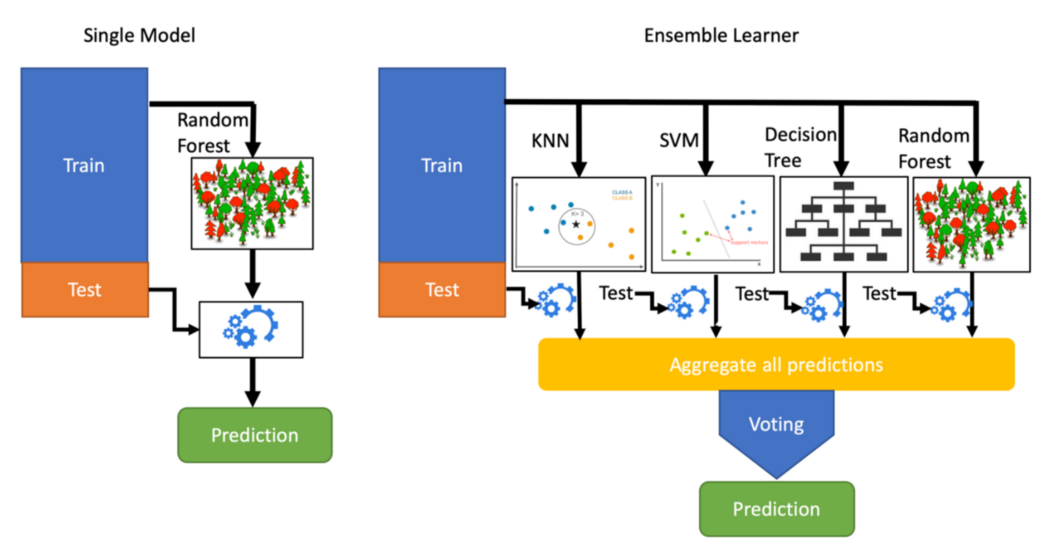
\includegraphics[scale=0.16]{ensemble-learning.png}
    \caption{Mô hình dự đoán đơn và mô hình tổng hợp \cite{An-xgboost}}
    \label{fig:ensemble-learning}
\end{figure}
\end{center}


Phương pháp học tổng hợp có thể thực hiện theo hai cách: Bagging (tổng hợp song song) hoặc Boosting (tổng hợp tuần tự). Trong bài này, chúng tôi chỉ tập trung vào Boosting do nó là nền tảng của XGBoost.

\subsection{Cách hoạt động của thuật toán Boosting}
Thuật toán Boosting mô hình yếu (weak learners) mới và kết hợp tuần tự các dự đoán của chúng để cải thiện hiệu suất tổng thể của mô hình. Đối với bất kỳ dự đoán sai nào, các mẫu phân loại sai sẽ được gán trọng số lớn hơn và các mẫu phân loại đúng sẽ được gán trọng số nhỏ hơn. Các mô hình học yếu (weak learner models) hoạt động tốt hơn có trọng số cao hơn trong mô hình tổng hợp cuối cùng. Boosting không bao giờ thay đổi dự đoán trước đó và chỉ sửa chữa những dự đoán tiếp theo bằng cách học hỏi những sai lầm. Vì Boosting sử dụng chiến lược tham lam, chúng ta nên đặt tiêu chí dừng như hiệu suất mô hình (dừng sớm) để ngăn chặn tình trạng quá khớp (overfitting) khi huấn luyện. 

\begin{center} 
\begin{figure}[!h]
    \centering
    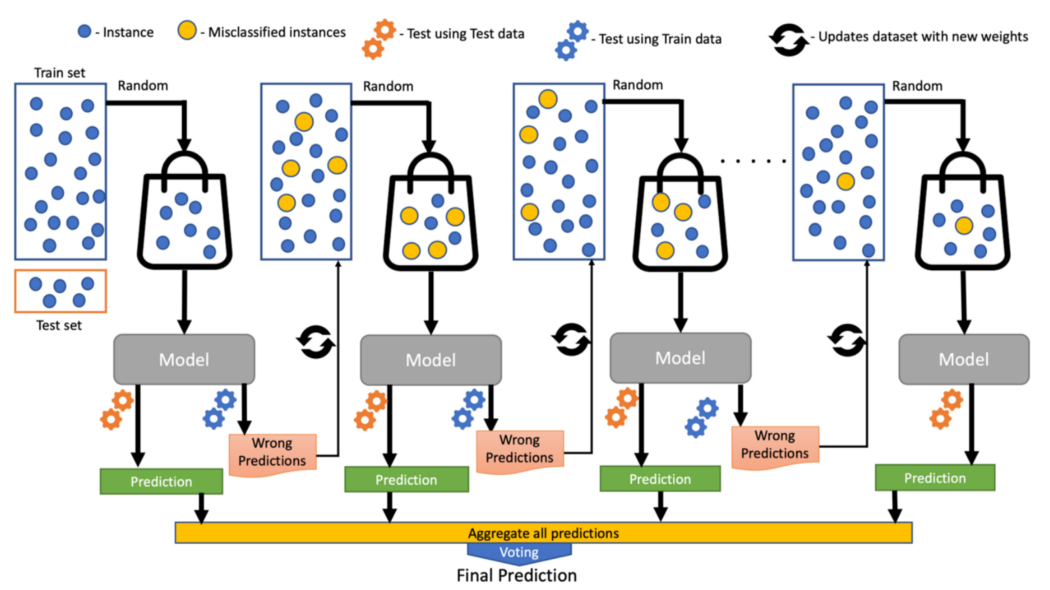
\includegraphics[scale=0.20]{boosting-algo.png}
    \caption{Cách thuật toán Boosting hoạt động \cite{An-xgboost}}
    \label{fig: boosting-algo}
\end{figure}
\end{center}

% /----------------------------------/
\section{Phương pháp} 
 
XGBoost, hay còn được biết đến với tên đầy đủ là  \textit{eXtreme Gradient Boosting}, là thuật toán máy học tổng hợp dựa trên cây quyết định (\textit{decision-tree-based ensemble learning algorithm}). XGBoost được phát triển bởi Tianqi Chen và hiện là một phần của bộ sưu tập thư viện mã nguồn mở rộng và đang được phát triển bởi Cộng đồng Máy học Phân tán (Distributed Machine Learning Community). Dù cho các mô hình mạng neural nhân tạo \cite{ANN} (\textit{artificial neural network}) có hiệu suất vượt trội hơn trên những tập dữ liệu phi cấu trúc như hình ảnh, âm thanh, những mô hình dựa trên cây quyết định thường sẽ chiếm ưu thế so với các mô hình mạng neural đối với dữ liệu có cấu trúc nhỏ hay các dữ liệu bảng biểu. 

\begin{center} 
\begin{figure}[!h]
    \centering
    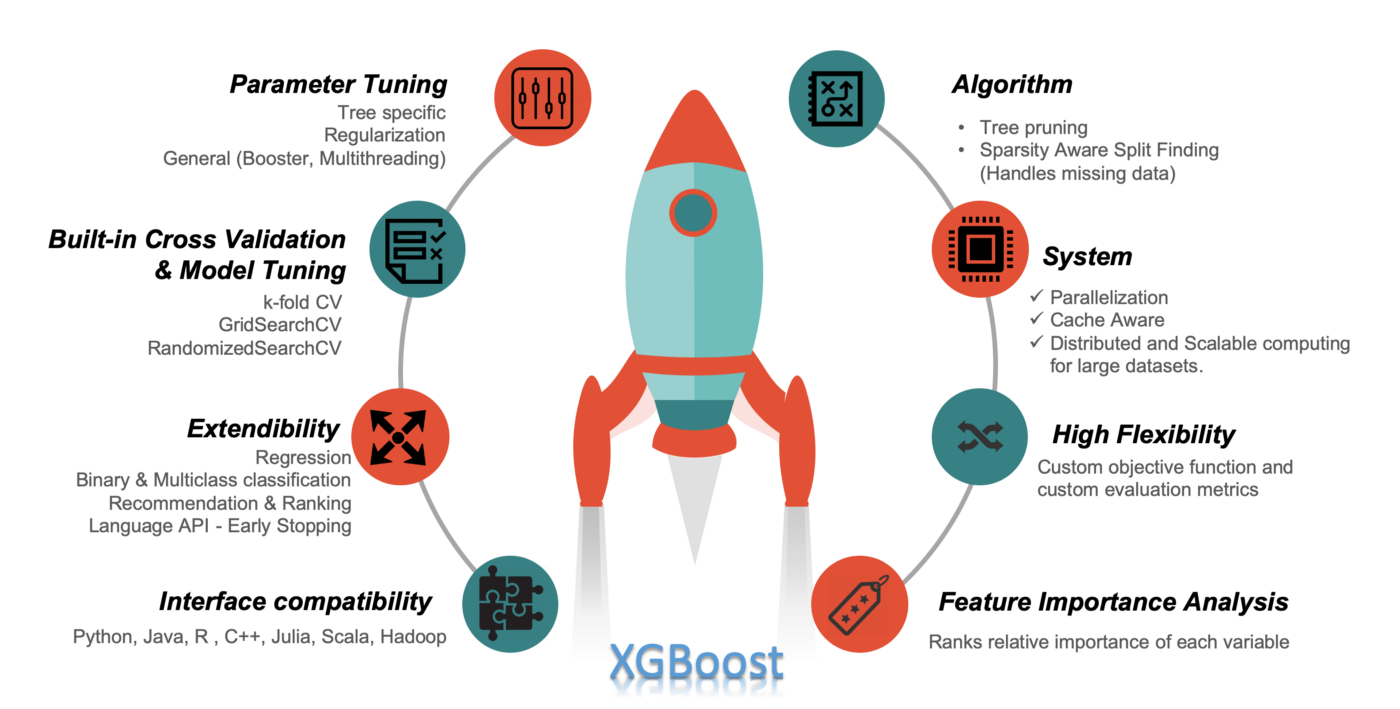
\includegraphics[scale=0.17]{xgboost-overview.png}
    \caption{Tổng quan về XGBoost \cite{An-xgboost}}
    \label{fig:xgboost-overview}
\end{figure}
\end{center}

\subsection{Sơ lược về các kĩ thuật phát triển XGBoost}
Dù cho hình thái đơn giản nhất của XGBoost - mô hình cây quyết định (\textit{decision tree}) rất dễ để ta có thể hình dung và hiểu được bản chất của thuật toán, việc phát triển nền tảng cho các mô hình tổng hợp dựa trên cây có phần khó khăn hơn thông qua việc sử dụng nhiều kĩ thuật khác nhau để xấp xỉ được dữ liệu đầu ra với độ lỗi là nhỏ nhất. Một vài kĩ thuật và thuật toán nổi bật trong việc phát triển các mô hình cây quyết định có thể được kể đến như:

\begin{itemize}  
    \item \textbf{Bagging}: là hướng tiếp cận sử dụng cơ chế bình chọn (voting) giữa tất cả các đặc trưng để có thể cho ra được dự đoán đầu ra cuối cùng.
    \item \textbf{Random Forest}: là thuật toán sử dụng cơ chế voting của bagging, tuy nhiên, Random Forest \cite{randomforest} chỉ sử dụng voting trên một số lượng đặc trưng nhất định được chọn ngẫu nhiên để đưa ra lựa chọn tốt nhất cho đầu ra của mình.
    \item \textbf{Boosting}: là hướng tiếp cận sử dụng cơ chế phản hồi (feedback) đến từ những lựa chọn đầu ra để gia tăng độ chính xác đầu ra của mô hình thông qua quá trình đánh giá tích cực (dynamic evaluation process).
    \item \textbf{Gradient Boosting}: là thuật toán boosting sử dụng gradient descent để tối thiểu hóa độ lỗi đầu ra nhưng không làm phức tạp hóa mô hình cây quyết định. Sự khác biệt giữa boosting và gradient boosting chính là cách thức cả hai thuật toán này cải thiện mô hình dựa trên những dự đoán lỗi.
\end{itemize}

\begin{center} 
\begin{figure}[!h]
    \centering
    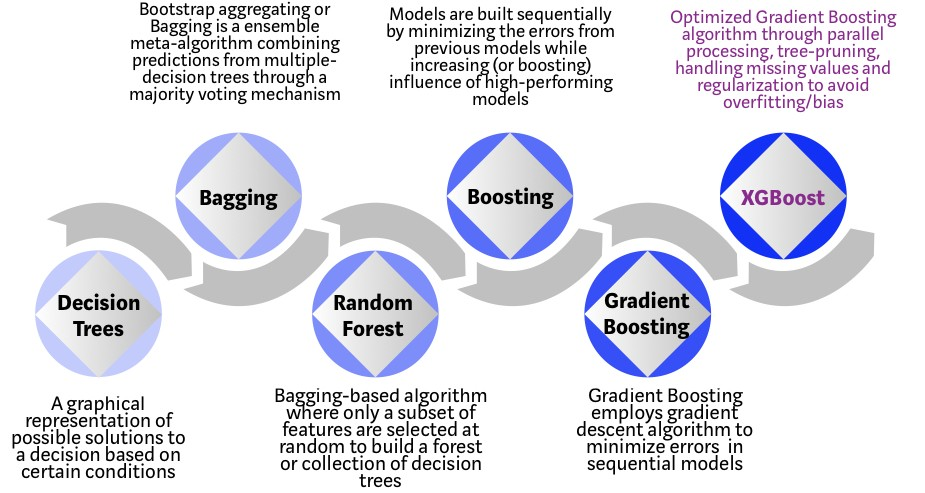
\includegraphics[scale=0.24]{evolution.jpeg}
    \caption{Sự tiến hoá của XGBoost bắt đầu từ mô hình cây quyết định \cite{An-xgboost}}
    \label{fig:evolution}
\end{figure}
\end{center}

\subsection{Ưu điểm của XGBoost}
Ưu điểm lớn nhất của XGBoost đó chính là việc XGBoost được thiết kế để giải quyết việc khuyết dữ liệu trong nội tại. Việc xử lí dữ liệu bị khuyết được thực hiện thông qua việc mô hình phát hiện và dự đoán xu hướng của dữ liệu bị thiếu trong tập dữ liệu đầu vào để có thể đưa ra được giá trị phù hợp cho phần khuyết đó. Cụ thể, XGBoost sẽ thử sai nhiều hướng tiếp cận khác nhau mỗi khi nó gặp một điểm dữ liệu bị thiếu ở mỗi node trên cây. Do đó, nó có khả năng giải quyết bài toán hợp lý hơn khi xử lý những dữ liệu không đầy đủ ở các giai đoạn sau (ví dụ trong giai đoạn kiểm tra hoặc giai đoạn triển khai phần mềm).

\begin{center} 
\begin{figure}[!h]
    \centering
    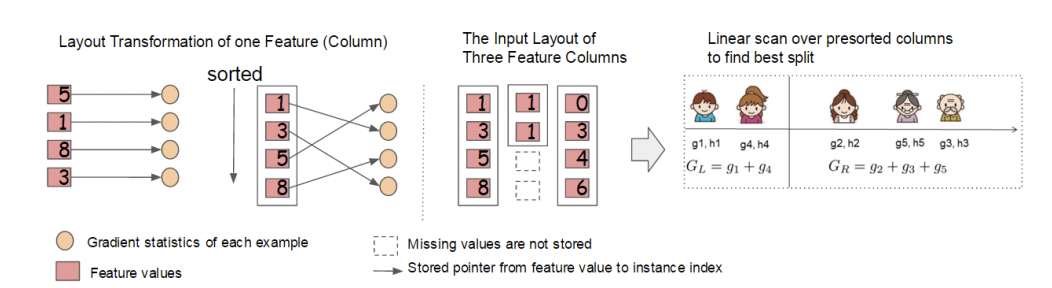
\includegraphics[scale=0.47]{parallel.png}
    \caption{Cấu trúc hình khối minh họa việc học song song (parallel learning) của XGBoost \cite{xgboost}}
    \label{fig:parallel}
\end{figure}
\end{center}

Ngoài ra, XGBoost còn có khả năng khai thác khả năng xử lý song song của máy tính và do đó nó có hiệu năng tính toán cao hơn rất nhiều so với các thuật toán GBM khác hay các thuật toán khác cùng dựa trên cây quyết định \cite{advantage_XGBoost}. Dù cho Boosting là một quá trình tuần tự, nó vẫn có khả năng tính toán song song. Mỗi cây quyết định trong XGBoost chỉ được tạo ra sau khi những cây cha (ancestor trees) của nó đã được tạo và tất cả các cây con có thể được xây dựng một cách đồng thời thông qua việc sử dụng toàn bộ nhân (core) của CPU. Điều này giúp cho XGBoost là một trong những thuật toán nhanh nhất trong họ các thuật toán dựa trên cây quyết định.

Một ưu điểm khác giúp XGBoost nổi trội hơn so với các thuật toán khác chính là nó cho phép người dùng có thể tự do tùy chỉnh những mục tiêu tối ưu và những độ đo trong việc đánh giá và xếp hạng những lời giải cho bài toán.

\begin{center} 
\begin{figure}[!h]
    \centering
    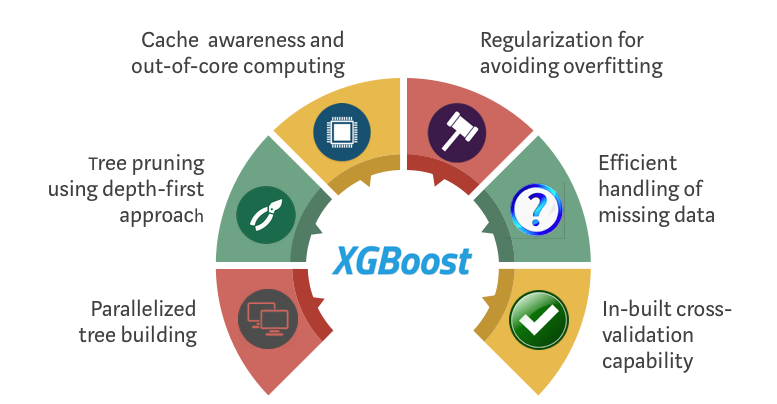
\includegraphics[scale=0.28]{optimize.png}
    \caption{Cách XGBoost tối ưu hoá thuật toán GBM tiêu chuẩn \cite{An-xgboost}}
    \label{fig:optimize}
\end{figure}
\end{center}
  
\subsection{Khuyết điểm của XGBoost} 

Dù XGBoost có nhiều lợi thế hơn so với các thuật toán khác nhưng nó vẫn còn tồn tại nhiều thiếu sót và bất cập trong việc triển khai cho nhiều loại bài toán cũng như nhiều loại dữ liệu khác nhau. Như đã đề cập, các kỹ thuật sử dụng mô hình mạng neural nhân tạo sẽ có độ chính xác ổn định và vượt trội hơn so với những thuật toán học máy khác như SVM \cite{svm}, AdaBoost \cite{adaboost}, Logistic Regression \cite{logisticregression} hay thậm chí là XGBoost. Cho đến nay, chỉ có những phương pháp học sâu mới có khả năng huấn luyện trên một lượng dữ liệu huấn luyện khổng lồ mà không bị bão hòa về mặt hiệu suất. Vì vậy, khi số lượng các mẫu huấn luyện trở nên rất lớn (chẳng hạn như 100.000 hay 1.000.000 mẫu) thì việc sử dụng các kỹ thuật học sâu sẽ mang lại hiệu quả cao hơn và tối ưu hơn về mặt thời gian.

Ngoài ra, dù XGBoost có độ chính xác cao hơn đối với đại đa số vấn đề và có các đặc tính tính toán tốt, nó không mang lại sự khác biệt đáng kể so với nhiều phương pháp truyền thống khác như SVM hoặc Random Forest, hay thậm chí có nhiều lúc hiệu suất của XGBoost trở nên cực kỳ tệ khi so sánh các thuật toán khác đơn giản hơn trong cùng một bài toán. Ta chỉ nên sử dụng mô hình XGBoost khi sở hữu một lượng đủ lớn (nhưng không quá lớn) các mẫu dữ liệu. Lý do là bởi vì mô hình này sẽ cố gắng tập trung vào mẫu dữ liệu mà người huấn luyện sẽ truyền vào, khi dữ liệu càng phong phú và đa dạng cũng như phạm vi các trường hợp hay đặc trưng lớn thì mô hình này có thể phát huy được tốt tác dụng của nó.
 
\subsection{Các siêu tham số quan trọng khi sử dụng XGBoost} 

Việc tìm hiểu về các tham số của một mô hình là rất quan trọng bởi vì chúng giúp người sử dụng (hay người lập trình) có thể dễ dàng chỉnh sửa cũng như tiến hành tinh chỉnh (tuning) các tham số để làm cho mô hình tốt hơn. Dưới đây, chúng tôi sẽ mô tả khái quát về một vài siêu tham số quan trọng để tối ưu hóa mô hình XGBoost:
 
Đầu tiên ta phải nhắc đến tham số \textbf{$n\_estimators$}. Khi huấn luyện các mô hình học sâu, chúng ta có một siêu tham số là số lượng epochs. Mỗi epoch là một lần chúng ta cho dữ liệu chạy qua mô hình. Tham số $n\_estimators$ của XGBoost cũng giống như số lượng epochs trong các mô hình học sâu. Ở mỗi epoch, thuật toán sẽ tiến hành sửa lỗi mà mô hình ở epoch trước mắc phải (hay còn được biết đến dưới dạng quy trình boosting).

Bên cạnh $n\_estimators$, chúng ta có thể cải thiện hiệu suất của XGBoost thông qua tham số $max\_depth$. Tham số này thường được sử dụng để xác định độ sâu của các cây quyết định trong mô hình học tổng hợp: độ sâu càng lớn thì sẽ giúp cho các dự đoán (hay các quyết định) của cây tốt hơn thông qua việc phức tạp hóa mô hình hiện có. Tuy nhiên, nếu độ sâu quá lớn sẽ khiến cho mô hình chúng ta bị quá khớp. 

Trong trường hợp dữ liệu chúng ta bị mất cân bằng (imbalanced data), XGBoost cung cấp phương thức để điều chỉnh độ cân bằng giữa các trọng số dương và các trọng số âm thông qua tham số siêu $scale\_pos\_weight$: nếu thuật toán chúng ta gặp trường hợp hội tụ sớm khi dữ liệu quá mất cân bằng, ta có thể cân nhắc điều chỉnh tham số này với một giá trị lớn hơn 0  hoặc có thể gán tham số này với giá trị là tỉ lệ giữa tổng các mẫu âm với tổng các mẫu dương ($\frac{\sum{\text{negative instances}}}{\sum{\text{positive instances}}}$)

Ngoài ra, XGBoost còn cho phép lập trình viên điều chỉnh thuật toán theo ý muốn thông qua việc cung cấp các phương thức như: phương pháp boosting sử dụng cho thuật toán (ví dụ như \textit{gbtree} hay \textit{dart} để xây dựng XGBoost dưới dạng các cây quyết định hay \textit{gblinear} để xây dựng XGBoost dưới dạng mô hình tuyến tính) hay điều chỉnh thuật toán xây dựng cây (\textit{auto} - tự tìm thuật toán xây dựng cây nhanh nhất thông qua hàm heuristic, \textit{exact} - sử dụng giải thuật tham lam, \textit{approx}, \textit{hist} - sử dụng biểu đồ tần suất (histogram) để tăng tốc việc xấp xỉ cây bằng giải thuật tham lam, hay thậm chí là \textit{gpu\_hist} - sử dụng GPU cho phương thức hist đã đề cập) thông qua việc lựa chọn tham số $booster$ và $tree\_method$ thích hợp.

Như bao mô hình học máy truyền thống khác, XGBoost cung cấp cho chúng ta phương thức để điều chỉnh tốc độ học trong quá trình huấn luyện thuật toán. Tham số để điều chỉnh tốc độ học cho thuật toán được xác định là tham số $eta$ hay $learning\_rate$: tốc độ học có tác dụng thay đổi tốc độ mô hình đi tìm cực trị khi ta tiến hành thực thi thuật toán, $eta$ càng thấp (trong khoảng $\left(0; 1\right)$) thì tốc độ mô hình đi tìm cực trị sẽ càng chậm, và $eta$ càng cao (trong khoảng $\left(1; +\infty\right)$) thì tốc độ mô hình đi tìm cực trị sẽ càng nhanh. Ta cần phải chọn giá trị $eta$ thích hợp mô hình vì nếu $eta$ quá cao thì mô hình khó có thể tìm được điểm cực trị gần với giá trị tối ưu. Tuy nhiên, nếu $eta$ quá thấp thì mô hình sẽ mất rất nhiều thời gian để có thể tìm đến với cực trị của bài toán.

Cuối cùng, XGBoost cũng cung cấp cho chúng ta cách xử lý khi thuật toán bị quá khớp trong giai đoạn kiểm thử. Khi mô hình XGBoost bị quá khớp, chúng ta có thể tiến hành chính quy hoá (regularization) mô hình để ràng buộc các hệ số với các chuẩn (norm) L1 và L2, tương tự với việc sử dụng mô hình Lasso và Ridge trong Hồi quy tuyến tính. Để thay đổi các hệ số chính quy hóa, ta sẽ tinh chỉnh tham số $alpha$ (với chuẩn L1) và tham số $lambda$ (với chuẩn L2). Việc sử dụng chuẩn L1 và L2 cho XGBoost sẽ mang lại ý nghĩa tương tự khi ta tiến hành giảm bậc của bài toán giúp cho bài toán trở nên đơn giản hơn. 

Ngoài việc sử dụng L1 và L2, ta còn có thể giúp cho mô hình tránh được tình trạng quá khớp thông qua việc sử dụng các tham số $subsample$. Ví dụ với $subsample = 0.5$, mô hình sẽ lựa chọn random $50\%$ mẫu trong dữ liệu ban đầu ra để huấn luyện. Ngoài ra, XGBoost còn các siêu tham số như $colsample\_bytree$, $colsample\_bylevel$ hay $colsample\_bynode$ để giúp cho mô hình tránh trường hợp quá khớp. Các siêu tham số trong lớp $subsample$ và $colsample$ thường sẽ nằm trong nửa đoạn $(0;1]$. Nếu ta tinh chỉnh các siêu tham số này ở mức vừa phải (dưới 0.5), mô hình XGBoost sẽ sử dụng ít đặc trưng và do đó tránh được tình trạng quá khớp. Tuy nhiên, cần phải lưu ý rằng nếu như ta tinh chỉnh các tham số này ở mức quá cao (trên 0.5), mô hình chúng ta sẽ dễ rơi vào tình trạng chưa khớp (underfitting).

Có thể thấy, XGBoost cung cấp cho ta rất nhiều sự lựa chọn để thay đổi các siêu tham số nhằm tùy biến mô hình. Tuy nhiên, chúng ta phải tinh chỉnh các siêu tham số ở mức hợp lý để đạt được độ chính xác hay mức độ điều hòa (harmonic) tốt.
% /--------------------------------------------------/
\section{Bộ dữ liệu}
\subsection{Mô tả dữ liệu}


% Những phương pháp mô phỏng hiện nay được huấn luyện dựa trên phương pháp cộng hưởng (ensemble), với mỗi mô hình sẽ mô phỏng tình trạng của một bên phổi khác nhau. Tuy nhiên, phổi và đặc điểm sinh học của phổi là một không gian biến liên tục, vì thế nên phương pháp tiếp cận như trên phải được cải tiến để có thể xét đến sự khác biệt giữa hai bên phổi của bệnh nhân.

% Nhóm nghiên cứu ở Google Brain và Đại học Princeton muốn tạo nên 1 cộng đồng máy học xung quanh vấn đề điều khiển tự động máy thở y tế này. Họ tin rằng mạng neural và học sâu có thể tổng quan hóa những đặc tính khác nhau của phổi tốt hơn so với những tiêu chuẩn hiện tại của bộ điều khiển PID ở thị trường hiện nay.


% Nếu thành công, chúng tôi sẽ vượt qua được trở ngại về giá thành trong việc phát triển nên những phương pháp mới trong việc điều khiển máy thở y tế. Điều này sẽ dẫn đường cho những thuật toán khác có thể thích nghi tốt với bệnh nhân và giảm đi gánh nặng về bệnh nhân của các bác sĩ trong thời điểm dịch tễ như hiện tại. Và qua đó, những phương pháp điều trị sử dụng máy thở y tế sẽ trở nên phổ biến rộng rãi hơn cho các bệnh nhân gặp vấn đề về đường hô hấp. 

% Dữ liệu về máy thở được sử dụng trong cuộc thi này được tạo ra bằng cách sử dụng một máy thở nguồn mở đã được sửa đổi kết nối với phổi kiểm tra ống thổi nhân tạo thông qua một mạch hô hấp. 

% Sơ đồ bên dưới minh họa cách thiết lập, với hai đầu vào điều khiển được đánh dấu màu xanh lá cây và biến trạng thái (áp suất đường thở) để dự đoán bằng màu xanh lam. Đầu vào điều khiển đầu tiên là một biến liên tục từ 0 đến 100 đại diện cho tỷ lệ phần trăm van điện từ của máy thở được mở để cho không khí vào phổi (nghĩa là $0$ đóng hoàn toàn không cho không khí vào và 100 mở hoàn toàn). Đầu vào điều khiển thứ hai là một biến nhị phân đại diện cho việc van thăm dò đang mở (1) hay đóng (0) để thoát khí ra ngoài.

% \begin{figure}[!h]
%   \centering
%   \includesvg[scale=0.18]{5.svg} 
% \end{figure}
 
Trong bài này, chúng tôi sử dụng bộ dữ liệu Ventilator Pressure Prediction của Google Brain\footnote{https://www.kaggle.com/c/ventilator-pressure-prediction}. Bộ dữ liệu này cung cấp thông tin về các chuỗi thời gian thở với mục tiêu là học cách dự đoán áp lực đường thở trong mạch hô hấp dựa trên những mốc thời gian khác nhau. 


Mỗi mốc thời gian đại diện cho một pha hô hấp kéo dài khoảng 3 giây. Bộ dữ liệu được sắp xếp sao cho mỗi hàng là một mốc thời gian của hơi thở và đưa ra hai tín hiệu điều khiển, kết quả là áp lực thở, cũng như các thuộc tính liên quan của phổi và máy thở, được mô tả chi tiết ở hình \ref{fig:mesh1}.\\

\begin{figure}[!h]
    \centering
    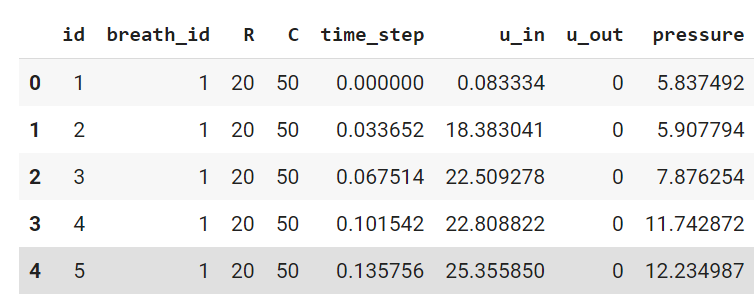
\includegraphics[scale=0.4]{1.png}
    \caption{Ví dụ về các thuộc tính trong 5 hàng đầu tiên của tập dữ liệu}
    \label{fig:mesh1}
\end{figure}
 
Trong đó:
\begin{itemize}
\item \textit{id} -- định danh mốc thời gian cho toàn bộ tập dữ liệu
\item \textit{breath\_id} -- định danh mốc thời gian giữa các pha hô hấp

\item \textit{R} -- thuộc tính phổi cho biết mức độ tắc nghẽn đường dẫn khí (có đơn vị là $cmH_{2}O / l / s$, trong đó: $l$ được kí hiệu cho lít và $s$ được kí hiệu cho giây). Về mặt vật lý, đây là sự thay đổi áp suất trên mỗi lần thay đổi lưu lượng phổi (lưu lượng thở trên một đơn vị thời gian). 

\item \textit{C} -- thuộc tính phổi cho biết mức độ giãn nở của phổi (có đơn vị là $mL / cmH_{2}O$). Về mặt vật lý, đây là sự thay đổi thể tích trên mỗi lần thay đổi áp lực thở. 
\item \textit{time\_step} -- mốc thời gian thực

\item \textit{u\_in} -- đầu vào điều khiển cho van điện tử hít vào (inspiratory solenoid valve), giá trị nằm trong phạm vi từ 0 đến 100.
\item \textit{u\_out} -- đầu vào điều khiển cho van điện từ thở ra (exploratory solenoid valve), mang giá trị 0 hoặc 1.
\item \textit{pressure} -- áp lực thở trong hệ hô hấp, tính bằng $cmH_2O$.
\end{itemize}



\subsection{Phân tích dữ liệu}
Để có cái nhìn chi tiết hơn về bộ dữ liệu, chúng tôi đã trực quan hóa mức độ tương quan giữa các thuộc tính thông qua biểu đồ nhiệt (heatmap) ở hình \ref{fig:correlation}.
% Ta có thể quan sát mức độ tương quan giữa các thuộc tính trong tập dữ liệu thông qua biểu đồ nhiệt (heatmap) như sau:
\begin{figure}[!h]
    \centering
    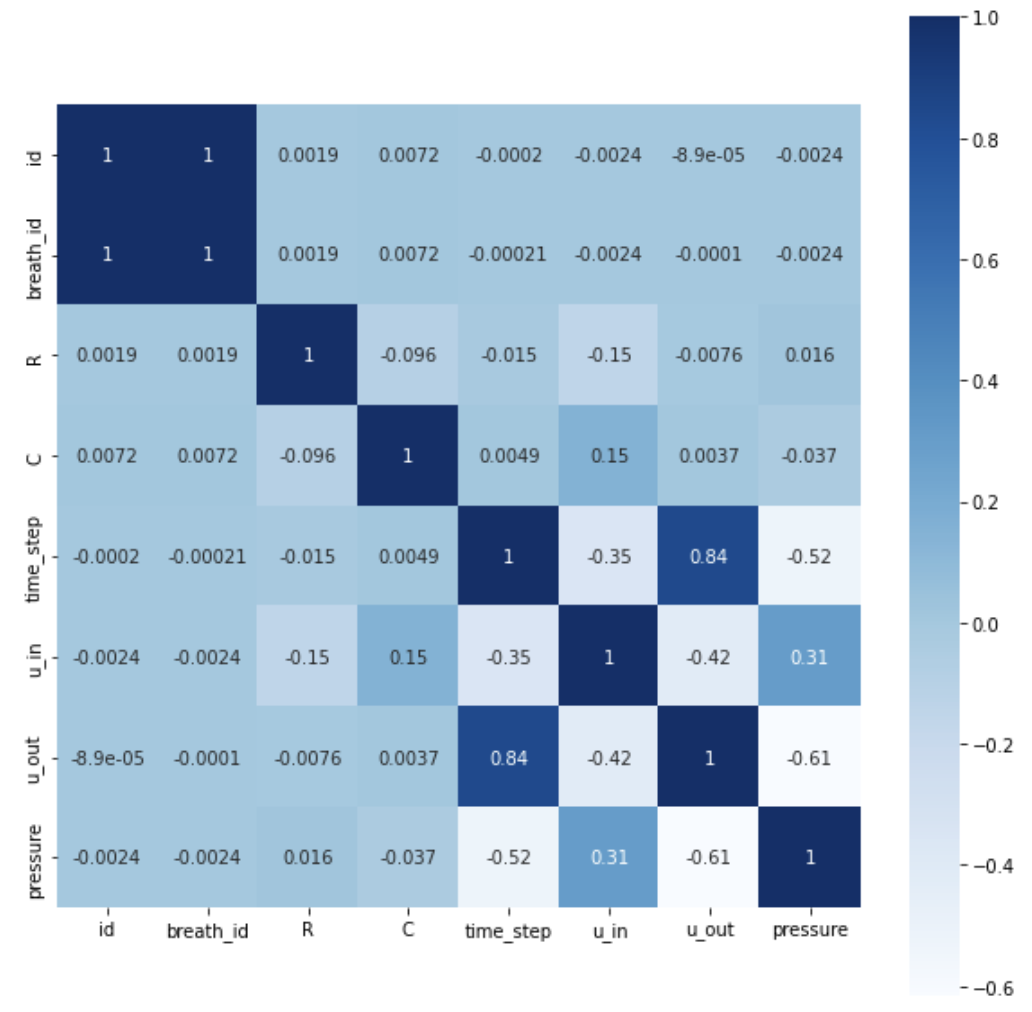
\includegraphics[scale=0.4]{correlation.png}
    \caption{Mức độ tương quan giữa các thuộc tính trong bộ dữ liệu}
    \label{fig:correlation}
\end{figure}

Ta có thể thấy được rằng: Ngoài hai tổ hợp đặc trưng id và breath\_id, hai đặc trưng có mức độ tương quan lớn nhất chính là time\_step và u\_out. Điều nay là bởi ta có thể quan sát được tiến trình hô hấp của bệnh nhân đang sử dụng máy thở (đang hít vào hay thở ra). 

\begin{figure}[h!]
  \centering 
  \begin{minipage}[b]{0.2\textwidth}
    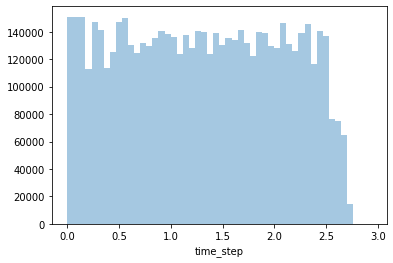
\includegraphics[width=\textwidth]{time_step.png}
    \caption{Tần số time\_step}
    \label{fig:time_step}
  \end{minipage}
  \hfill
  \begin{minipage}[b]{0.2\textwidth}
    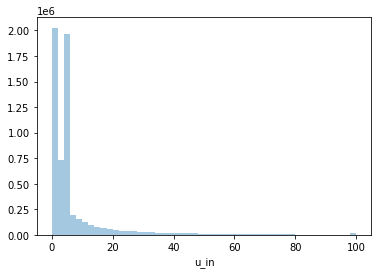
\includegraphics[width=\textwidth]{u_in.png}
    \caption{Tần số u\_in}
    \label{fig:u_in}
  \end{minipage}
\end{figure}

\begin{figure}[h!]
  \centering
  \begin{minipage}[b]{0.2\textwidth}
    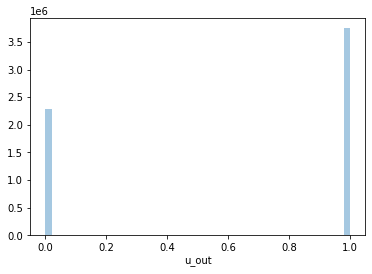
\includegraphics[width=\textwidth]{u_out.png}
    \caption{Tần số u\_out}
    \label{fig:u_out}
  \end{minipage}
  \hfill
  \begin{minipage}[b]{0.2\textwidth}
    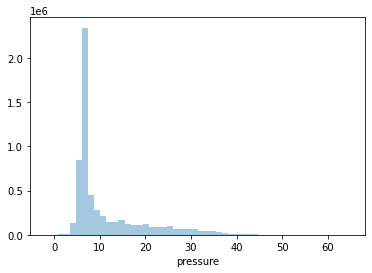
\includegraphics[width=\textwidth]{pressure.png}
    \caption{Tần số pressure}
    \label{fig:pressure}
  \end{minipage}
\end{figure}

Ngoài ra, đặc trưng pressure cũng có một sự phụ thuộc khá cao vào đặc trưng u\_in. Điều này có thể được lý giải thông qua nguyên lý của máy thở: khi ta thay đổi giá trị của u\_in, nghĩa là ta đang thay đổi áp suất không khí có trong phế quản của bệnh nhân, tương ứng với giá trị của biến số pressure trong tập dữ liệu. 

Bên cạnh pressure, thuộc tính $C$ cũng có mức độ phụ thuộc đáng kể với u\_in. Khi ta tăng hay giảm giá trị của van điện tử hít vào, mức độ giãn nỡ của phổi cũng sẽ thay đổi theo (biến đổi theo thể tích không khí truyền vào phổi). Những đặc trưng còn lại có mức độ tương quan thấp hoặc không đáng kể lẫn nhau. 

Bên cạnh mức độ tương quan, ta còn có thể hiểu rõ hơn về cách phân bố dữ liệu thông qua một số đồ thị histogram như ở hình \ref{fig:time_step}, \ref{fig:u_in}, \ref{fig:u_out} và \ref{fig:pressure}.

% Tại đây chúng tôi sẽ phân tích sơ lược về cách phân bố của dữ liệu huấn luyện. Tại hình \ref{fig:time_step} có thể thấy rằng dữ liệu được tổ chức phân bố khá đồng đều, tuy nhiên ở những phần cuối cùng thì mật độ của $time\_step$ lại giảm dần. Dù vậy những điều này cũng sẽ không quá ảnh hướng đến mô hình vì đại đa số chúng đều được phân bố đều và rải rác xung ở những phần phía trước. Trái ngược với nó, phần mô tả phân bố dữ liệu ở hình \ref{fig:u_out} lại không như vậy. Có thể thấy một cách rõ ràng rằng số lượng phần tử mang giá trị $1$ nhiều hơn hẳn so với số lượng phần tử mang giá trị $0$ ở thuộc tính $u\_out$ trong bảng dữ liệu được cung cấp. 

% Bên cạnh đó, khi quan sát $2$ thuộc tính $u\_in$ và $pressure$ ở hình \ref{fig:u_in} và hình \ref{fig:pressure} thì lại lại thu được một mức tương đồng khá giống nhau. Cả hai thuộc tính đều có mức bộ phân bố dày đặc ở phần phía trước sau đó lại cùng nhau giảm dần về phía phải của đồ thị. Chính vì vậy mà mức độ tương quan của hai thuộc tính này được đánh giá khá cao. 

% /--------------------------------------------------/

\section{Thực nghiệm}

% Chúng tôi chia tập dữ liệu ra thành hai tập train và test với tỉ lệ lần lượt là 70\% và 30\%.

% Sau khi quan sát các phân phối của dữ liệu được cung cấp, chúng tôi quyết định chạy thực nghiệm mô hình XGBoost với các tham số ban đầu như sau: 
% \begin{itemize} 
%     \item $n\_estimators = 5000$ -- số lần ước lượng của mô hình.
%     \item $learning\_rate$ $(lr)$ $= 0.9$ -- tốc độ học của mô hình. 
%     \item $subsample = 0.95$ -- Tỉ lệ mẫu con để huấn luyện là $95\%$.
%     \item $colsample\_bytree$ $(\text{cols/tree})$ $= 0.5$ -- Tỷ lệ mẫu của các cột khi xây dựng mỗi cây.
%     \item $max\_depth$ $(d_{max})$ $= 2$ -- Độ sâu tối đa của cây khi huấn luyện. 
%     \item $booster =$ 'gbtree'
%     \item $reg\_lambda$ $(\text{reg}_\lambda)$ $= 66.1$ -- Chính quy hóa dạng $L1$.
%     \item $reg\_alpha$ $(\text{reg}_\alpha)$ $= 15.9$ -- Chính quy hóa dạng $L2$. 
%     \item $random\_state = 42$ 
%     \item $tree\_method =$ 'gpu\_hist'
%     \item $gpu\_id = 0$
%     \item $predictor =$ 'gpu\_predictor'
% \end{itemize} 
% % \begin{table}[]
% % \begin{tabular}{|l|l|l|}
% % \hline
% % Parameters              & Value  & Description                     \\ \hline
% % n\_estimators           & 5000   & số lần ước lượng của mô hình    \\ \hline
% % learning\_rate          & 0.9    & Tốc độ học của mô hình          \\ \hline
% % subsample               & 0.95   & Tỷ lệ mẫu được huấn luyện       \\ \hline
% % colsample\_bytree       & 0.5    & Tỷ lệ mẫu của các cột ở mỗi cây \\ \hline
% % max\_depth (d\_{max}) & 2      & Độ sâu tối đa của cây           \\ \hline
% % booster                 & gbtree &                                 \\ \hline
% % reg\_lambda             & 66.1   & Chính quy hóa dạng L1           \\ \hline
% % reg\_alpha              & 15.9   & Chính quy hóa dạng L2           \\ \hline
% % \end{tabular}
% % \end{table}

% Ngoài ra, trong quá trình huấn luyện, chúng tôi sử dụng phương pháp K-Fold cross-validation \cite{kfold} nhằm đánh giá mô hình một cách hiệu quả. Bên cạnh đó, chúng tôi cũng tiến hành chạy thực nghiệm nhằm chọn ra $k$ tốt nhất cho phương pháp K-Fold cross validation.
 
% \begin{figure}[!h]
%     \centering
%     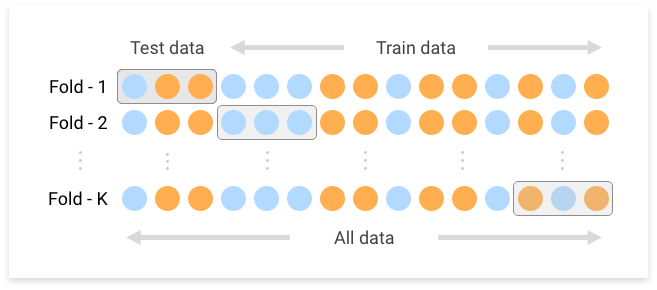
\includegraphics[scale=0.34]{KFold.png}
%     \caption{Hình ảnh mô phỏng quá trình thực nghiệm bằng phương pháp K-Fold}
%     \label{fig:mesh2}
% \end{figure}

% % Khi chạy thực nghiệm sử dụng phương pháp 5-folds, chúng tôi thu kết quả $score=0.63816$ chính là trung bình của 5 lần sau khi huấn luyện mô hình. 

% \begin{center}
%     \begin{tikzpicture}
%         \begin{axis}[
%             title={Kiểm định 10 lần mô hình trên phương pháp KFold},
%             xlabel={Fold},
%             ylabel={Độ chính xác},
%             xmin=1, xmax=10,
%             ymin=0.635, ymax=0.64,
%             xtick={1, 2, 3, 4, 5, 6, 7, 8, 9, 10},
%             ytick={0.635, 0.6375, 0.64},
%             legend pos=north west,
%             ymajorgrids=true,
%             grid style=dashed,
%         ]
%         \addplot[color=blue,mark=square,]
%             coordinates {
%             (1, 0.636936) (2, 0.637288) (3, 0.638114) (4, 0.637305) (5, 0.637855)
%             (6, 0.639075) (7, 0.637508) (8, 0.638530) (9, 0.639975) (10, 0.639017) 
%             };
%             \legend{loss}
            
%         \end{axis}
%     \end{tikzpicture}
% \end{center} 

% Từ biểu đồ trên có thể thấy với việc mô hình sử dụng K-Fold cross-validation với $k = 10$, kết quả thu được tương đối đồng đều và khá tốt, không có sự chênh lệch khá lớn mà độ lệch chuẩn chỉ rơi vào khoảng $0.7$. 

% Để đạt được hiệu quả cao nhất, chúng tôi đã tiến hành sử dụng phương pháp Grid Search nhằm tìm ra bộ siêu tham số phù hợp nhất cho mô hình. 
 
% \begin{table}[!h]
% \caption {Bảng hiển thị quá trình tuning các tham số} 
% \begin{tabular}{|l|l|l|l|l|l|l|l|}
% \hline
%  & lr & cols/tree &d$_{max}$&reg$_\lambda$&reg$_\alpha$ & train & test \\ \hline
% 1 & 0.9 & 0.5 & 2 & 66.1& 15.9 & 0.72 & 5.99 \\ \hline
% 2 & 1.9 & 0.5 & 2 & 66.1 & 15.9 & \textbf{0.72} & 9.74\\ \hline
% 3 & 0.5 & 0.5 & 2 & 66.1 & 15.9 & 0.72 & \textbf{4.98} \\ \hline
% 4 & 0.5 & 0.5 & 2 & 80 & 30 & \textbf{0.72} & \textbf{4.68} \\ \hline
% 5 & 0.5 & 0.5 & 2 & 100 & 50 & 0.72 & 5.15 \\ \hline
% 6 & 0.5 & 0.5 & 3 & 80 & 30 & 0.75 & 5.75 \\ \hline
% 7 & 0.5 & 0.1 & 2 & 80 & 10 & \textbf{0.64} & 5.55 \\ \hline
% 8 & 0.5 & 0.5 & 2 & 70 & 20 & \textbf{0.63} & \textbf{4.70}  \\ \hline
% \end{tabular}
% \end{table} 

% Đầu tiên chúng ta sẽ thử nghiệm ngẫu nhiên các tham số và thu được kết quả khá khả quan với xấp xỉ loss trên tập train và tập test lần lượt là $0.72$ và $5.99$. Sau đó chúng tôi tiến hành bước tinh chỉnh tham số $learning\_rate$ lên $1.9$ nhằm khiến mô hình học nhanh hơn, tuy nhiên việc lại lại khiến cho loss của tập $test$ lại tăng lên đáng kể (hơn $1.95$). Đến lần tinh chỉnh tham số thứ ba, chúng tôi thay giá trị của $learning\_rate$ từ $1.9$ trở thành $0.5$ (tức là giảm đi $0.4$ so với lần đầu tiên và thu được kết quả lạc quan hơn tại tập test với loss xấp xỉ $4.98$ giảm $1.01$ so với loss tại lần một. Nhận thấy rằng hai giá trị $reg\_lambda$ và $reg\_alpha$ vẫn còn nhỏ ( khiến mô hình XGBoost học chưa đủ nghiêm ngặt), chúng tôi đã chỉnh sửa lại hai tham số trên từ $66.1$, $15.9$ thành $80$, $30$ và thu được kết quả cải thiện hơn lần thử trước khoảng $4.68$ (tốt hơn $0.3$).

\subsection{Thang đo}
Trong quá trình thực nghiệm, chúng tôi sử dụng thang đo là \textit{sai số tuyệt đối trung bình} (Mean Absolute Error). Đây là một phương pháp đo lường sự khác biệt giữa hai biến liên tục. Giả sử rằng X và Y là hai biến liên tục thể hiện kết quả dự đoán của mô hình và kết quả thực tế. chúng ta có độ đo MAE được tính theo công thức sau:

\begin{equation}
    MAE = \frac{1}{n}\sum_{i=1}^{n}{| y_{i} - x_{i} |} 
\end{equation} 

Trong đó, $n$ là số lượng điểm dữ liệu, $x_i$ là giá trị thực của tập huấn luyện tại điểm thứ $i$, $y_i$ là giá trị dự đoán tại điểm thứ $i$.

Độ đo này thường được sử dụng để đánh giá sự sai khác giữa mô hình dự đoán và tập kiểm tra trong các bài toán hồi quy. Chỉ số này càng nhỏ thì mô hình học máy càng chính xác.

\subsection{Chi tiết triển khai}
Chúng tôi sử dụng phương pháp Tìm kiếm theo lưới (Grid Search) \cite{gridsearch} để lựa chọn các siêu tham số cho XGBoost. Tìm kiếm theo lưới là một kỹ thuật tinh chỉnh các siêu tham số để tìm ra bộ siêu tham số tối ưu nhất. Đây là một kỹ thuật tìm kiếm vét cạn được thực hiện trên một không gian tìm kiếm cụ thể được định nghĩa trước. Tìm kiếm theo lưới tuy đơn giản nhưng lại giúp chúng ta tiết kiệm thời gian, công sức và tài nguyên.

Nhằm đánh giá XGBoost một cách hiệu quả nhất, chúng tôi tiến hành so sánh XGBoost với một số mô hình như Linear Regression và LightGBM \cite{lightgbm}. Bên cạnh đó, chúng tôi cũng sử dụng kỹ thuật K-Fold Cross Validation và Grid Search cho cả ba thuật toán XGBoost, Light GBM và Hồi quy tuyến tính (Linear Regression).

Sau khi chạy Grid Search chúng tôi quyết định lựa chọn các siêu tham số của LightGBM và XGBoost như sau:

\begin{center}
    \begin{table}[h!]
    \begin{tabular}{|c|c|}
        \hline
        Siêu tham số & Giá trị \\
        \hline 
        booster & 'gbtree' \\
        \hline 
        gamma & 3.2\\
        \hline 
        gpu\_id & 0 \\
        \hline
        learning\_rate & 0.1\\
        \hline 
        max\_depth & 8 \\
        \hline 
        n\_estimators & 5000\\
        \hline 
        predictor & 'gpu\_predictor' \\
        \hline 
        reg\_alpha & 15.9 \\
        \hline 
        reg\_lambda & 66.1\\
        \hline 
        subsample & 0.95\\ 
        \hline 
        tree\_method & 'gpu\_hist'\\
        \hline
    \end{tabular}
    \caption{Siêu tham số được sử dụng cho XGBoost}
    \label{tab: table-xgboost} 
    \end{table}
\end{center}

\begin{center}
    \begin{table}[h!]
    \begin{tabular}{|c|c|}
        \hline
        Siêu tham số & Giá trị \\
        \hline 
        bagging\_fraction & 1.0\\
        \hline 
        bagging\_freq & 0\\
        \hline 
        boosting\_type & 'gbdt' \\
        \hline
        feature\_fraction & 0.90\\
        \hline 
        feature\_pre\_filter & False\\
        \hline 
        lambda\_l1 & 0.0\\
        \hline 
        lambda\_l2 & 0.0 \\
        \hline 
        learning\_rate & 0.1 \\
        \hline 
        max\_depth & 8\\
        \hline 
        metric & 'l1'\\ 
        \hline 
        min\_child\_samples & 2\\
        \hline
        num\_leaves & 350\\
        \hline 
        objective & 'regression\_l1'\\
        \hline 
        random\_state & 42\\ 
        \hline 
        verbose & -1\\
        \hline
    \end{tabular}
    \caption{Siêu tham số được sử dụng cho LightGBM}
    \label{tab: table-lightgbm} 
    \end{table}
\end{center}

\subsection{Kết quả}

\begin{center}
    \begin{table}[h!]
    \begin{tabular}{|c|c|c|}
        \hline
        Thuật toán & MAE & Thời gian huấn luyện (s) \\
        \hline 
        XGBoost  & 4.6240 & 148.32  \\
        \hline 
        LightGBM & 4.7457  & 30.9537 \\
        \hline 
        Hồi quy tuyến tính &  8.09 & 1.46 \\
        \hline
    \end{tabular}
    \caption{Sai số tuyệt đối trung bình và thời gian huấn luyện của ba thuật toán: XGBoost, LightGBM và Linear Regression}
    \label{tab: table-1} 
    \end{table}
\end{center}



% bagging_fraction': 1.0, 
% 'bagging_freq': 0, 
% 'boosting_type': 'gbdt', 
% 'feature_fraction': 0.8999999999999999, 
% 'feature_pre_filter': False, 
% 'lambda_l1': 0.0, 
% 'lambda_l2': 0.0, 
% 'learning_rate': 0.1, 
% 'max_depth': 8, 
% 'metric': 'l1', 
% 'min_child_samples': 2, 
% 'num_leaves': 350, 
% 'objective': 'regression_l1', 
% 'random_state': 42, 
% 'verbose': -1

Kết quả cuối cùng chúng tôi đạt được trên tập kiểm tra (Bảng \ref{tab: table-1}) cho thấy tuy XGBoost có thời gian huấn luyện lâu nhất nhưng vẫn ở mức chấp nhận được. Đổi lại, XGBoost đạt được MAE tốt nhất so với hai thuật toán LgihtGBM và Hồi quy tuyến tính. Bên cạnh đó, LightGBM cũng cho thấy mình là một đối thủ đáng gờm với XGBoost khi có MAE thua kém không đáng kể và thời gian huấn luyện vượt trội. Ngoài ra, chúng tôi cũng khảo sát một mô hình đơn giản là Hồi quy tuyến tính (Linear Regrression) nhưng kết quả không tốt lắm dù thời gian huấn luyện chỉ hơn 1 giây.

\subsection{Triển khai ứng dụng}
Để chứng minh tính ứng dụng của nghiên cứu này, chúng tôi có phát triển một ứng dụng web bằng NodeJS cho phép người dùng nhập vào các đặc trưng như trong bộ dữ liệu và đầu ra là áp lực của máy thở lên bệnh nhân. Video demo được công khai tại: \url{https://github.com/DTA-UIT/Ventilator_Pressure_Prediction}

% /--------------------------------/
\section{Bàn luận}
\subsection{Có nên sử dụng XGBoost mọi lúc, mọi nơi?}
Câu trả lời dĩ nhiên là không. Khi giải quyết một bài toán bằng học máy, chúng ta phải kiểm tra tất cả các thuật toán có thể trên một tập dữ liệu được cho sẵn mới có thể khẳng định được thuật toán nào là tốt nhất. Bên cạnh đó, việc lựa chọn đúng thuật toán là chưa đủ. Chúng ta còn phải lựa chọn bộ siêu tham số phù hợp cho thuật toán đó và điều này là không hề dễ dàng với những thuật toán có nhiều siêu tham số cũng như có phạm vi tìm kiếm siêu tham số rộng. Ngoài ra vẫn còn nhiều yếu tố khác để lựa chọn thuật toán như độ phức tạp, khả năng giải thích và tính khả thi khi triển khai. Do vậy, khi đụng phải một bài toán, chúng ta vẫn phải suy nghĩ xem là nên lựa chọn thuật toán nào dựa vào những điều trên chứ không nên sử dụng cố định một thuật toán nào đó.

\subsection{XGBoost liệu có thể giữ vững được vị thế của mình?}
Trí tuệ nhân tạo là một lĩnh vực luôn luôn vận động và phát triển. Do đó, đã có không ít các giải pháp được đề xuất để thay thế cho XGBoost. Năm 2016, Microsoft đã cho ra mắt thuật toán LightGBM và nó đã nhanh chóng cho thấy một tiềm năng rất lớn. CatBoost của Yandex ra mắt năm 2017 cũng mang lại những kết quả rất ấn tượng. Dù các thuật toán này chưa thể đánh bại được XGBoost hoàn toàn nhưng để một thuật toán nào đó có thể có hiệu năng vượt trội hơn XGBoost thì vấn đề chỉ là thời gian mà thôi. Tuy vậy, cho đến khi kẻ thách thức mới xuất hiện thì XGBoost vẫn là kẻ thống trị thế giới học máy.
% /--------------------------------/

\section{Kết luận}
Trong nghiên cứu này, chúng tôi cũng đã làm rõ được những lý thuyết nền tảng của XGBoost cũng như phân tích một số khía cạnh của bộ dữ liệu. Ngoài ra, chúng tôi đã tiến hành so sánh XGBoost với một số thuật toán khác như LightGBM và Hồi quy tuyến tính trên tập dữ liệu dự đoán áp lực của máy thở lên bệnh nhân. Qua những kết quả thu được, XGBoost đã thể hiện hiệu năng tốt nhất so với các thuật toán khác cũng như đạt được thời gian huấn luyện chỉ hơn 2 phút.

% /--------------------------------/
\section*{Lời cảm ơn}
Chúng tôi chân thành gửi lời cảm ơn đến TS. Nguyễn Vinh Tiệp đã giảng dạy môn Lập trình Python cho Máy học cũng như đưa ra những lời góp ý giúp chúng tôi chỉnh sửa bài báo cáo này.
\bibliographystyle{plain}
\bibliography{main_ref}

\end{document}

